%https://www.maa.org/sites/default/files/images/upload_library/46/Pengelley_projects/Project-11/430lame.pdf
\subsection{Euler-Catalan recurrence}
\begin{python0}
from solutions import *; clear() 
\end{python0}


Here are two very famous problems: the triangulation problem
and the parenthesizing problem.
The two problems are related.

Historically, the triangulation problem appears first, i.e.,
the counting of the number of ways $t_n$ to triangulate a convex $n$--sided
polygon,
and was first proposed by Euler in letter dated 1751 to Goldbach.
(Goldbach was Euler’s mentor.)
The whole subject surrounding counting triangulations has a
long and interesting history.

Euler found a closed form for $t_n$ back in 1751.
This was purely from computing $t_n$ up to $n = 25$.
However he couldn't prove its correctness.
Later, in 1758, Segner discovered a recurrence relation
for $t_n$ but he couldn't find a connection between his recurrence
relation to Euler's closed form.
In 1838, Lam\'e finally proved Euler's closed was correct.
So altogether from Euler's discovery of a possible closed form
for triangulation counting to the discovery of proof of correctness took more
than 80 years!

Back in 1758, after Segner found his recurrence for $t_n$,
Segner computed $t_n$ up to $n = 20$.
Euler checked Segner's calculation and found that Segner
made an error in his computation at $n = 15$.
(Which is why I already said that computation with
recurrences is slower and and hence
very error prone -- one would prefer to use a closed form!)
But since Segner's calculation of agreeing with Euler's computation
of $t_n$ up to $n = 14$, it's very likely that
Euler realized the value of Segner's recurrence relation.
Using Segner's recurrence relation, it's very likely that
in 1758 Euler was able to prove that his closed form is
correct by using the method of generating functions (which
requires Segner's recurrence).
If he did, then he probably never found time to publish
his proof.

The numbers $C_n$ in the second problem are called
\defone{Catalan numbers} and are closely related to the
triangulation numbers.
Catalan's contribution to these two problems is actually
minimal when compared to Euler, Segner, and Lam\'e.
Research triangulations and the Catalan numbers is still very active
to this day.

\begin{ex}
  Let $n \geq 3$ and let $t_n$ be the number of ways to triangulate a convex
  polygon
  with $n$ vertices.
  A convex polygon is a polygon where if you draw a line between any two
  vertices of the polygon, this line is in the polygon (and not outside).
  Here's a triangulation for the case of $n = 6$:
  
\begin{center}

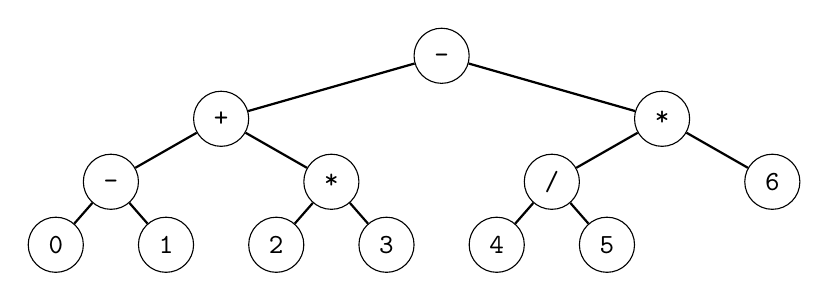
\begin{tikzpicture}
\node at (4.8999999999999995,-0.8) [circle,draw,minimum size=7mm] (A) {\texttt{-}};
\node at (2.0999999999999996,-1.6) [circle,draw,minimum size=7mm] (B) {\texttt{+}};
\node at (7.699999999999999,-1.6) [circle,draw,minimum size=7mm] (C) {\texttt{*}};
\node at (0.7,-2.4000000000000004) [circle,draw,minimum size=7mm] (D) {\texttt{-}};
\node at (3.5,-2.4000000000000004) [circle,draw,minimum size=7mm] (E) {\texttt{*}};
\node at (6.3,-2.4000000000000004) [circle,draw,minimum size=7mm] (F) {\texttt{/}};
\node at (9.1,-2.4000000000000004) [circle,draw,minimum size=7mm] (G) {\texttt{6}};
\node at (0.0,-3.2) [circle,draw,minimum size=7mm] (H) {\texttt{0}};
\node at (1.4,-3.2) [circle,draw,minimum size=7mm] (I) {\texttt{1}};
\node at (2.8,-3.2) [circle,draw,minimum size=7mm] (J) {\texttt{2}};
\node at (4.199999999999999,-3.2) [circle,draw,minimum size=7mm] (K) {\texttt{3}};
\node at (5.6,-3.2) [circle,draw,minimum size=7mm] (L) {\texttt{4}};
\node at (7.0,-3.2) [circle,draw,minimum size=7mm] (M) {\texttt{5}};
\draw [-,thick] (A) -- (B);
\draw [-,thick] (A) -- (C);
\draw [-,thick] (B) -- (D);
\draw [-,thick] (B) -- (E);
\draw [-,thick] (C) -- (F);
\draw [-,thick] (C) -- (G);
\draw [-,thick] (D) -- (H);
\draw [-,thick] (D) -- (I);
\draw [-,thick] (E) -- (J);
\draw [-,thick] (E) -- (K);
\draw [-,thick] (F) -- (L);
\draw [-,thick] (F) -- (M);

;
\end{tikzpicture}
    
\end{center}


  (Triangulation is a very important step in geometric computations
  and appears in areas
  such as computer graphics, computer vision, geographic information
  systems, etc.)
\end{ex}



\begin{ex}
  let $C_n$ be the number of ways to fully parenthesize a product of
  $n + 1$ symbols.
  For instance when $n = 4$,
  here's one way to parenthesize $x_0 x_1 x_2 x_3 x_4$:
  \[
    x_0 ((x_1 (x_2 x_3)) x_4)
  \]
  The fully parenthesized expression will then allow you to compute
  the product.
  ($C_n$ will then tell you how many possible ways to compute the
  product, which will tell you how many cases you would need to analyze
  before actually caring out the multiplications.
  This is important for instance in matrix chain multiplications
  where different parenthesizing gives rise to very different runtimes.
  See CISS358.)
\end{ex}

\newpage
\subsection*{Solutions}

\newpage
\section*{Solutions}
Solution to Exercise \ref{ex:power-series-11}\labeltext{}{sol:power-series-11}.

\debug{\tinysidebar{exercises/{power-series-11/answer.tex}}}
 
(a) From
\begin{align*}
\sum_{n = 0}^\infty \frac{1}{2^n} x^n \cdot \sum_{n = 0}^\infty \frac{1}{2^n} x^n
&=
\left(
1 + \frac{1}{2}x + \frac{1}{4}x^2 + \frac{1}{8}x^3 + \cdots
\right)
\left(
1 + \frac{1}{2}x + \frac{1}{4}x^2 + \frac{1}{8}x^3 + \cdots
\right)
\end{align*}
the coefficient of $x^3$ is
\[
1 \cdot \frac{1}{8}
+ \frac{1}{2} \cdot \frac{1}{4}
+ \frac{1}{4} \cdot \frac{1}{2}
+ \frac{1}{8} \cdot 1
= 4 \cdot \frac{1}{8} = \frac{1}{2}
\]
The coefficient of $x^n$ is
\[
\sum_{k=0}^n \frac{1}{2^k} \cdot \frac{1}{2^{n-k}}
= \sum_{k=0}^n \frac{1}{2^k \cdot 2^{n-k}}
= \sum_{k=0}^n \frac{1}{2^n}
= \frac{n + 1}{2^n}
\]

(b)
First let's derive the coefficient of $x^n$ in general. 
The coefficient of $x^n$ is
\begin{align*}
\sum_{k=0}^n \frac{1}{2^k} \cdot \frac{1}{3^{n-k}}
&= \sum_{k=0}^n \frac{1}{2^k} \cdot \frac{3^k}{3^n} 
= \frac{1}{3^n} \sum_{k=0}^n \left(\frac{3}{2}\right)^k \\
&= \frac{1}{3^n} \cdot \frac{1 - (3/2)^{n+1}}{1 - 3/2} \\
&= \frac{1}{3^n} \cdot \frac{1 - (3/2)^{n+1}}{-1/2} \\
&= \frac{1}{3^n} \cdot \frac{(3/2)^{n+1} - 1}{1/2} \\
&= \frac{2}{3^n} \cdot \left( \frac{3^{n+1}}{2^{n+1}} - 1 \right) \\
&= 2 \cdot \left( \frac{3^{n+1} - 2^{n+1}}{2^{n+1}3^n} \right) \\
&= \frac{3^{n+1} - 2^{n+1}}{6^n}
\end{align*}
The coefficient of $x^3$ is
\[
\frac{3^4 - 2^{4}}{6^4} = \frac{65}{216}
\]



\newpage

Solution to Exercise \ref{ex:power-series-15}\labeltext{}{sol:power-series-15}.

\debug{\tinysidebar{exercises/{power-series-15/answer.tex}}}
We have
\begin{align*}
\left( \sum_{n=0}^\infty x^n \right)^{100} 
&= \left( \frac{1}{1 - x} \right)^{100} \\
&= \sum_{n=0}^\infty \binom{100 + n - 1}{n} x^n \\
&= \sum_{n=0}^\infty \binom{n + 99}{n} x^n \\
&= \sum_{n=0}^\infty \binom{n + 99}{99} x^n
\end{align*}
Hence the coefficient of $x^n$ is $\binom{n + 99}{99} x^n$ for $n \geq 0$.


\newpage

Solution to Exercise \ref{ex:power-series-16}\labeltext{}{sol:power-series-16}.

\debug{\tinysidebar{exercises/{power-series-16/answer.tex}}}

We have
\begin{align*}
&\left( 
2 + 5x + \frac{7}{1 - x}
\right)
\left( \sum_{n=0}^\infty x^n \right)^{100}
\\
&= \left( 
2 + 5x + \frac{7}{1 - x}
\right)
\left( \frac{1}{1 - x} \right)^{100}
\\
&=
2\left( \frac{1}{1 - x} \right)^{100}
+ 5x \left( \frac{1}{1 - x} \right)^{100}
+ \frac{7}{1 - x} \left( \frac{1}{1 - x} \right)^{100}
\\
&=
2 \sum_{n=0}^\infty \binom{100 + n - 1}{n} x^n
+ 5x \sum_{n=0}^\infty \binom{100 + n - 1}{n} x^n
+ 7 \left( \frac{1}{1 - x} \right)^{101} 
\\
&=
2 \sum_{n=0}^\infty \binom{n + 99}{n} x^n
+ 5x \sum_{n=0}^\infty \binom{n + 99}{n} x^n
+ 7 \sum_{n=0}^\infty \binom{101 + n - 1}{n}
\\
&=
\sum_{n=0}^\infty 2 \binom{n + 99}{99} x^n
+ \sum_{n=0}^\infty 5 \binom{n + 99}{99} x^{n+1}
+ \sum_{n=0}^\infty 7 \binom{n + 100}{n} x^n
\\
&=
\sum_{n=0}^\infty 2 \binom{n + 99}{99} x^n
+ \sum_{p=1}^\infty 5 \binom{p + 98}{99} x^{p}
+ \sum_{n=0}^\infty 7          \binom{n + 100}{n} x^n  \,\,\, \text{(let $p = n + 1$)}
\\
&=
\sum_{n=0}^\infty 2\binom{n + 99}{99} x^n
+ \sum_{n=1}^\infty 5 \binom{n + 98}{99} x^{n}  
+ \sum_{n=0}^\infty 7 \binom{n + 100}{100} x^n \,\,\,\text{(replace $p$ by $n$)}
\\
&=
2 \binom{99}{99} + \sum_{n=1}^\infty 2\binom{n + 99}{99} x^n
+ \sum_{n=1}^\infty 5\binom{n + 98}{99} x^{n} 
+ 7\binom{100}{100}  + \sum_{n=1}^\infty 7 \binom{n + 100}{100}  
\\
&=
9 +
\sum_{n=1}^\infty
\left( 2\binom{n + 99}{99} 
+  5\binom{n + 98}{99} 
+ 7 \binom{n + 100}{100}
\right) x^n
\end{align*}
Hence the coefficient of $x^n$ is
\[
\begin{cases}
9 & \text{ if } n = 0 \\
\displaystyle 2\binom{n + 99}{99} 
+  5\binom{n + 98}{99} 
+ 7 \binom{n + 100}{100} & \text{ if } n > 0
\end{cases}
\]


\newpage

Solution to Exercise \ref{ex:power-series-17}\labeltext{}{sol:power-series-17}.

\debug{\tinysidebar{exercises/{power-series-17/answer.tex}}}

(a)
\begin{align*}
\sum_{n=0}^\infty \frac{1}{2^n} x^n
\cdot
\sum_{n=0}^\infty \frac{1}{2^n} x^n
&=
\left( \sum_{n=0}^\infty \frac{1}{2^n} x^n \right)^2
\\
&=
\left( \sum_{n=0}^\infty \left( \frac{x}{2} \right)^n \right)^2
\\
&=
\left( \sum_{n=0}^\infty \left( \frac{x}{2} \right)^n \right)^2
\\
&=
\left( \frac{1}{1 - (x/2)} \right)^2
\\
&=\sum_{n=0}^\infty \binom{2 + n - 1}{n} \left( \frac{x}{2} \right)^n
\\
&=\sum_{n=0}^\infty \binom{n + 1}{n} \left( \frac{1}{2} \right)^n x^n
\\
\sum_{n=0}^\infty \left( \frac{n + 1}{2^n} \right x^n
\end{align*}

(b)
\begin{align*}
\sum_{n=0}^\infty \frac{1}{2^n} x^n
\cdot
\sum_{n=0}^\infty \frac{1}{3^n} x^n
\end{align*}
    

 % input solutions.tex
